\glsresetall{}
\chapter{Introduction}
Despite the incessant progress over the last seventy years, there are still many problems today’s computers cannot solve in a realistic amount of time. While some calmly await the next generation of supercomputers, others might remain intractable for classical computers forever.

Theoretical physicist Richard Feynman popularized this observation in the early eighties. In particular, he argued that classical computers could not simulate quantum mechanics efficiently~\cite{Feynman1982SimulatingComputers}. Based on the pioneering work of Ed Fredkin and Tomasso Toffoli~\cite{Fredkin1982ConservativeLogic}, he proposed an alternative computation model exploiting fundamental properties of quantum mechanics. %Quantum computers were born --- at least, on paper.

The following decade saw a plethora of developments in quantum algorithms and quantum information 
theory~\cite{Deutsch1992RapidComputation,Shor1995Polynomial-TimeComputer,Grover1996ASearch,Simon1997OnComputation, Bernstein1997QuantumTheory,Bennett1997StrengthsComputing}. Consequently, potential applications emerged in several other fields such as information security, machine learning and optimization. In this thesis, we focus on optimization and implement an algorithm that finds an approximate solution to a combinatorial problem.

This introduction, which consists of five sections, provides the necessary material to understand the subsequent chapters. The first section introduces fundamental concepts of quantum computing and quantum information. The second provides an overview of how to realize a quantum computing experiment with superconducting circuits, the technology used in our experiments. The third section describes the constraints of near-term quantum computing resulting from imperfect implementation and suggests ways to mitigate their effect: (i) using variational quantum algorithms (VQAs) and (ii) using a more expressive gate set tailored to VQAs, thereby avoiding decomposition in their quantum circuits implementations. The fourth section further details the principles of VQAs and illustrates why the controlled arbitrary phase gate, which we implement in this thesis, is a suitable gate to avoid decomposition. Finally, the last section reports on related work and introduces the scientific contributions of this work. 

\section{Quantum computing} \label{sec:intro_quantum_computing}
Both classical and quantum computing aspire to the same goal: solving problems with algorithms. However, they differ fundamentally in the way they represent information. Classical computers encode information in binary variables, called (classical) bits. At any point in time, a bit has a state of either 0 or 1. Quantum computers rely on a generalization of this concept: the quantum bit, referred to as \textit{qubit}. A qubit has a \textit{quantum state}, $\ket{\psi}$, which, like a classical bit, is characterized by two basis states, \0 and \1\footnote{$\ket{\cdot}$ is the Dirac notation for state vectors, often used in quantum mechanics.}. However, unlike its classical counterpart, during a computation, a qubit can adopt any linear combination of these two basis states:
\begin{equation}
|\psi\rangle=\alpha|0\rangle+\beta|1\rangle, \quad \{\alpha, \beta\} \in \mathbb{C}
\end{equation}
where $\alpha, \beta$ are the (complex) amplitudes of the basis states \0 and \1, respectively. We say that the qubit can be in a \textit{superposition} of the two basis states. 

Unfortunately, quantum mechanics postulates it is impossible to examine (i.e. measure) the amplitudes of a quantum state directly. Instead, a single measurement projects the states onto only \textit{one} of the basis states with a probability equal to the squared modulus of its amplitude. In the one-qubit case, $\ket{\psi}$ yields \0 with probability $|\alpha|^2$ and \1 with probability $|\beta|^2$ and $|\alpha|^2 + |\beta|^2 = 1$. Nevertheless, it is the leveraging of interference between these amplitudes within the quantum algorithm (i.e.~\textit{before} measuring) that makes quantum computing particularly powerful.

Several qubits put together form a quantum state with even more basis states, each of which has its own amplitude. For instance, a two-qubit system encodes the quantum state $|\psi'\rangle=\alpha|00\rangle+\beta|01\rangle+\gamma|10\rangle+\delta|11\rangle$, with 4 basis states and 4 amplitudes. Generally speaking, a $N$-qubit system has $2^N$ basis states and can be in a superposition of all of them.

In close analogy to how logical gates (e.g. NOT, AND, OR) act on bits to perform classical computations, quantum algorithms consist of individual operations implemented via quantum gates, acting on single or multiple qubits. These quantum gates take a quantum state as input, shuffle the amplitudes and outputs a modified quantum state. For instance, a single-qubit gate can take $|\psi\rangle=\alpha|0\rangle+\beta|1\rangle$ and exchange the amplitudes $\alpha$ and $\beta$ such that the output is $|\phi\rangle=\beta|0\rangle+\alpha|1\rangle$. This is analogous to what a NOT gate would do to a classical bit. 

There is a convenient mathematical way to visualize how a quantum gate acts on a quantum state. Namely, using vectors and matrices. In the single qubit case, a state $|\psi\rangle=\alpha|0\rangle+\beta|1\rangle$ is encoded into the vector $\transpose{(\alpha, \beta)}$ while the gate $G$ is represented as a unitary\footnote{A complex square matrix $U$ is unitary if its conjugate transpose $U^\dagger$ is also its inverse, i.e.\ if $U^\dagger U=U U^\dagger=I$.} $2\times2$ matrix, 
\begin{equation}
G = 
\begin{pmatrix}
a_0 & a_1 \\
b_0 & b_1
\end{pmatrix}
\end{equation}
in which the coefficients in the first and second column indicate how the gate affects the basis states \0 and \1 respectively. In particular, if the input state is \0, which can be written as $ \transpose{(1,0)}$, then the output state is $a_0\ket0 + b_0\ket1$ and if the input state is \1 then the output state is $a_1\ket0 + b_1\ket1$. In the more general case, if the input state is $\ket\psi = \transpose{(\alpha, \beta)}$, then the output state $\ket\phi$ is given by the product
\begin{equation}
    \ket\phi = G \ket \psi = 
    \begin{pmatrix}
a_0 & a_1 \\
b_0 & b_1
\end{pmatrix} \cdot 
\begin{pmatrix}
\alpha \\
\beta 
\end{pmatrix}
\end{equation}
For the single-qubit gate exchanging $\alpha$ and $\beta$, $G = \left(\transpose{(0,1)}, \transpose{(1,0)}\right)$ such that
\begin{equation}
\ket\phi = G \ket \psi = 
\begin{pmatrix}
0 & 1 \\
1 & 0
\end{pmatrix} \cdot 
\begin{pmatrix}
\alpha \\
\beta 
\end{pmatrix} =  
\begin{pmatrix}
\beta \\
\alpha 
\end{pmatrix}
\end{equation}
A similar technique is used for two-qubit gates. They are described by $4\times4$ matrices multiplying vectors with 4 entries (one for each basis state).

Remarkably, a very small set of single- and two-qubit gates, called \textit{universal gate set}, is sufficient to implement any quantum computation with arbitrarily many qubits because any high level instruction can be decomposed to a list of gates belonging to that universal gate set~\cite{Nielsen2000QuantumInformation}\footnote{A similar concept also exists in classical computing, stating that NAND gates alone form a universal set.}.

The existence of universal gate sets is very valuable for building a quantum computer because it implies we can perform quantum computation with few distinct gates implemented in hardware. Nevertheless, building a quantum computer remains an immense challenge. Indeed, it requires to create and manipulate objects displaying quantum mechanical properties, which typically do not materialize at the scale we live in. One option, as we shall see in the next section, consists in mimicking atoms and their quantum mechanical properties with superconducting circuits.

\section{Quantum computers with superconducting circuits} \label{sec:intro_building_qc}
Since the advent of quantum information theory, many technologies have been explored to build quantum computers: ions trapped in an electromagnetic trap~\cite{Monroe1995DemonstrationGate}, semiconductor quantum dots~\cite{Loss1998QuantumDots}, photons and linear optics~\cite{Knill2001AOptics}, superconducting circuits~\cite{Blais2004CavityComputation}, and many more. While each technology has its pros and cons, in this thesis we focus on superconducting circuits, one of the leading technology platform ~\cite{Kjaergaard2019SuperconductingPlay} which we use in our experiments.

In superconducting circuits, qubits are represented by artificial atoms, realized as superconducting electrical circuits with discrete energy levels. Typically, the first two levels are chosen to represent the basis states \0 and \1  while the remaining ones are ignored. The core idea is to create a quantum harmonic oscillator using an $LC$-circuit ($L$ is an inductor and $C$ is a capacitor). This circuit has a resonance frequency $\omega = 1/\sqrt{LC}$ which corresponds to the frequency of the transition between the energy levels in the system. In a quantum mechanical picture, the resulting harmonic potential has quantized energy levels spaced by the energy quantum $\hbar\omega$~\cite{Kjaergaard2019SuperconductingPlay}, where $\hbar$ is the reduced Planck constant. 

Provided the temperature is sufficiently low and there is little dissipation, the energy levels of the oscillator are distinguishable and addressable. However, the equidistant spacing between energy levels prevents from using directly the quantum harmonic oscillator as a qubit. Indeed, while trying to induce a transition from \0 to \1 by injecting an energy quantum, we might induce a transition from \1 to \2 if there is already an excitation in the system. Hence, we cannot restrict the computational space to the first two levels as desired for binary quantum computing. 

To circumvent this problem, we create an anharmonic energy potential by using a non-linear inductor called a Josephson tunnel junction~\cite{Vion2003QuantumProcessing}. The junction's inductance depends non-linearly on the magnetic flux flowing through it. The introduced anharmonicity enables the separate addressing of each transition with the  matching transition frequency. 

There are several ways to obtain a Hamiltonian with discretized, anharmonic energy levels using a Josephson junction. One of them consist in creating a superconducting island with one side connected to ground via a Josephson junction, and the other coupled via a capacitor to a voltage source~\cite{Bouchiat1998QuantumPair, Nakamura1999CoherentBox}. 

When the voltage source is unbiased, the system lies in the ground state, \0, also referred to as \g. By increasing the voltage of the source, we polarize the island with the capacitor until a charge quantum\footnote{These charge quanta are called Cooper-pairs and form at very low temperature when two electrons of opposite spin in the metal pair up to form a bosonic state. At sufficiently low temperatures, all valence electrons in the metal form Cooper-pairs and they can all occupy the same ground state.} tunnels (without loss) through the Josephson junction onto the island to restore charge balance. The energy stored in the capacitor after the tunneling is called the charging energy, $E_C$, and the energy stored in the junction is called the Josephson energy, $E_J$. 
If the gate voltage is subsequently removed, there is \textit{charge offset} on the island and the system is out of equilibrium, i.e., there is one excitation in the system (\1 or \e). Because the state of the system depends on the amount of charge on the island, this implementation is called the \textit{charge qubit}.

In our experiments, we use the \textit{transmon}~\cite{KochCharge-insensitiveBox} -- a special case of the charge qubit -- that operates in the regime $E_J/E_C \approx 50$ to mitigate environmental charge noise~\cite{KochCharge-insensitiveBox, Oliver2013MaterialsBits}. In addition, we use a SQUID to control the Josephson energy with an external magnetic flux, $\Phi$.
The total energy required to introduce excitations in the system depends on the energies $E_J(\Phi)$ and $E_C$. For the first transition energy~\cite{KochCharge-insensitiveBox},
\begin{equation} \label{eq:qubit_frequency}
    E_{\ket{1}}/\hbar \approx \omega_{\ket{1}} \approx \sqrt{8E_J(\Phi) E_C} - E_C
\end{equation}

Transition frequencies for frequency tunable transmons are typically located in the micro-wave part of the electromagnetic spectrum (4-8 GHz). Therefore, we use microwave pulses tuned to the appropriate transition frequency to perform the single-qubit gates between the state \0 and \1.

Due to the inherent environmental noise, implementing perfect quantum gates represents an immense challenge in practice. Other experimental considerations further complicate the implementation of quantum computing: for instance, \textit{decoherence}, the process of loosing quantum information encoded in a system over time due to undesirable interactions with the environment\footnote{We typically distinguish between \textit{relaxation}, characterized by the time constant \t{1}, which relates to the spontaneous decay of excitation captured in the system after some time, and \textit{dephasing}, characterized by the time constant \t{2}$^{*}$ , which relates to the loss of information about the phase of the system.}, puts a hard bound how many quantum operations can be executed reliably. 
In addition, information stored in qubits cannot be copied~\cite{Wootters1982ACloned} which prevents the use of cloning and majority voting as error correcting scheme. Instead, quantum error correction codes employing many physical qubits to encode the state of few logical qubits~\cite{Gottesman2010AnComputation, DiVincenzo1996Fault-TolerantCodes, Fowler2012SurfaceComputation} are required to achieve fault-tolerant quantum computing. 

These experimental complications will impose limitations on what (noisy) quantum computers achieve in the near future. Nevertheless, the steady improvement of coherence times and multi-qubit chip control over the last two decades now enable quantum computations which challenge the most powerful classical supercomputers~\cite{Arute2019QuantumProcessor}.  We are thus at the dawn of a new and exciting quantum computing stage that physicists have named the \textit{noisy intermediate-scale quantum} era.

\section{The noisy intermediate-scale quantum era}
While Google recently claimed having performed a task on a 53-qubit quantum computer that would take extremely long time on a supercomputer~\cite{Arute2019QuantumProcessor}, full-scale fault-tolerant quantum computing is still a distant dream. The pivotal period we just entered, called the \gls{nisq} era~\cite{Preskill2018QuantumBeyond}, entails two major limitations on near-term quantum computers:
\begin{enumerate}
    \item The performance of quantum devices is severely limited by noise. There are many possible sources of noise. However, a dominant one is decoherence. For fixed coherence times, quantum computers can only execute a limited number of operations (quantum gates) before quantum information is lost. We say that decoherence limits the \textit{depth} of the quantum circuit.
    \item The number of qubits available for computation is limited. Fabricating high quality and multi-qubit quantum processors is a laborious task. Therefore, we expect near-term quantum computers to have fewer than 1000 physical qubits.
\end{enumerate} 

Bearing in mind those limitations, how can we make best use of current quantum computers? 

Firstly, we shall implement quantum algorithms, such as \textit{\glspl{vqa}}~\cite{Moll2017QuantumDevices}, which are believed to cope better with \gls{nisq} limitations. \Glspl{vqa} are suited for the \gls{nisq} era because they outsource part of the algorithm which does not require quantum properties to classical computers. Therefore, available qubits are used more efficiently and part of the computation is carried out by classical computers which do not suffer from decoherence. In addition, \glspl{vqa} are intrinsically less sensitive to noise because they seek approximate solutions (instead of exact solutions). Hence, coherent errors may be partially compensated for by the classical optimizer such that they lead to worse approximate solutions but typically do not ruin the whole computation. Nonetheless, errors accumulating over time (such as decoherence) will severely limit the performance of \glspl{vqa}.

Secondly, we  can significantly reduce the time required to execute \glspl{vqa} on quantum computers by tailoring the available gate set on the quantum computer to match typical operations performed by \glspl{vqa}. The conceptual underlying principle is presented in Fig.~\ref{fig:intro_quantum_circuits}. When generating a quantum circuit to solve a mathematical problem, the first step consists of formulating the problem we want to solve in a way which the \gls{vqa} can take it as input. Next, we receive a list of instructions from the algorithm to follow in order to solve the problem. These instructions are passed on to the quantum computer. However, the quantum computer can only perform a restricted set of operations based on the available gates implemented in hardware. Therefore, it might be necessary to decompose some operations into a longer sequence of available gates.

In particular, decomposition occurs when a \gls{vqa} is implemented on a quantum computer with a so-called standard gate set. This set comprises of the most commonly implemented two-qubit gates such as the CNOT-, CZ- and SWAP-gate. They receive most attention because a small subset of them, such as the CNOT-gate (or SWAP-gate) combined with arbitrary single-qubit gates, forms a universal gate set which allows to implement any instruction, as discussed in Section~\ref{sec:intro_quantum_computing}. However, the decomposition of these instructions can be arbitrarily long, which is a major drawback, especially during the \gls{nisq} era.

\begin{figure}[ht]
    \centering
    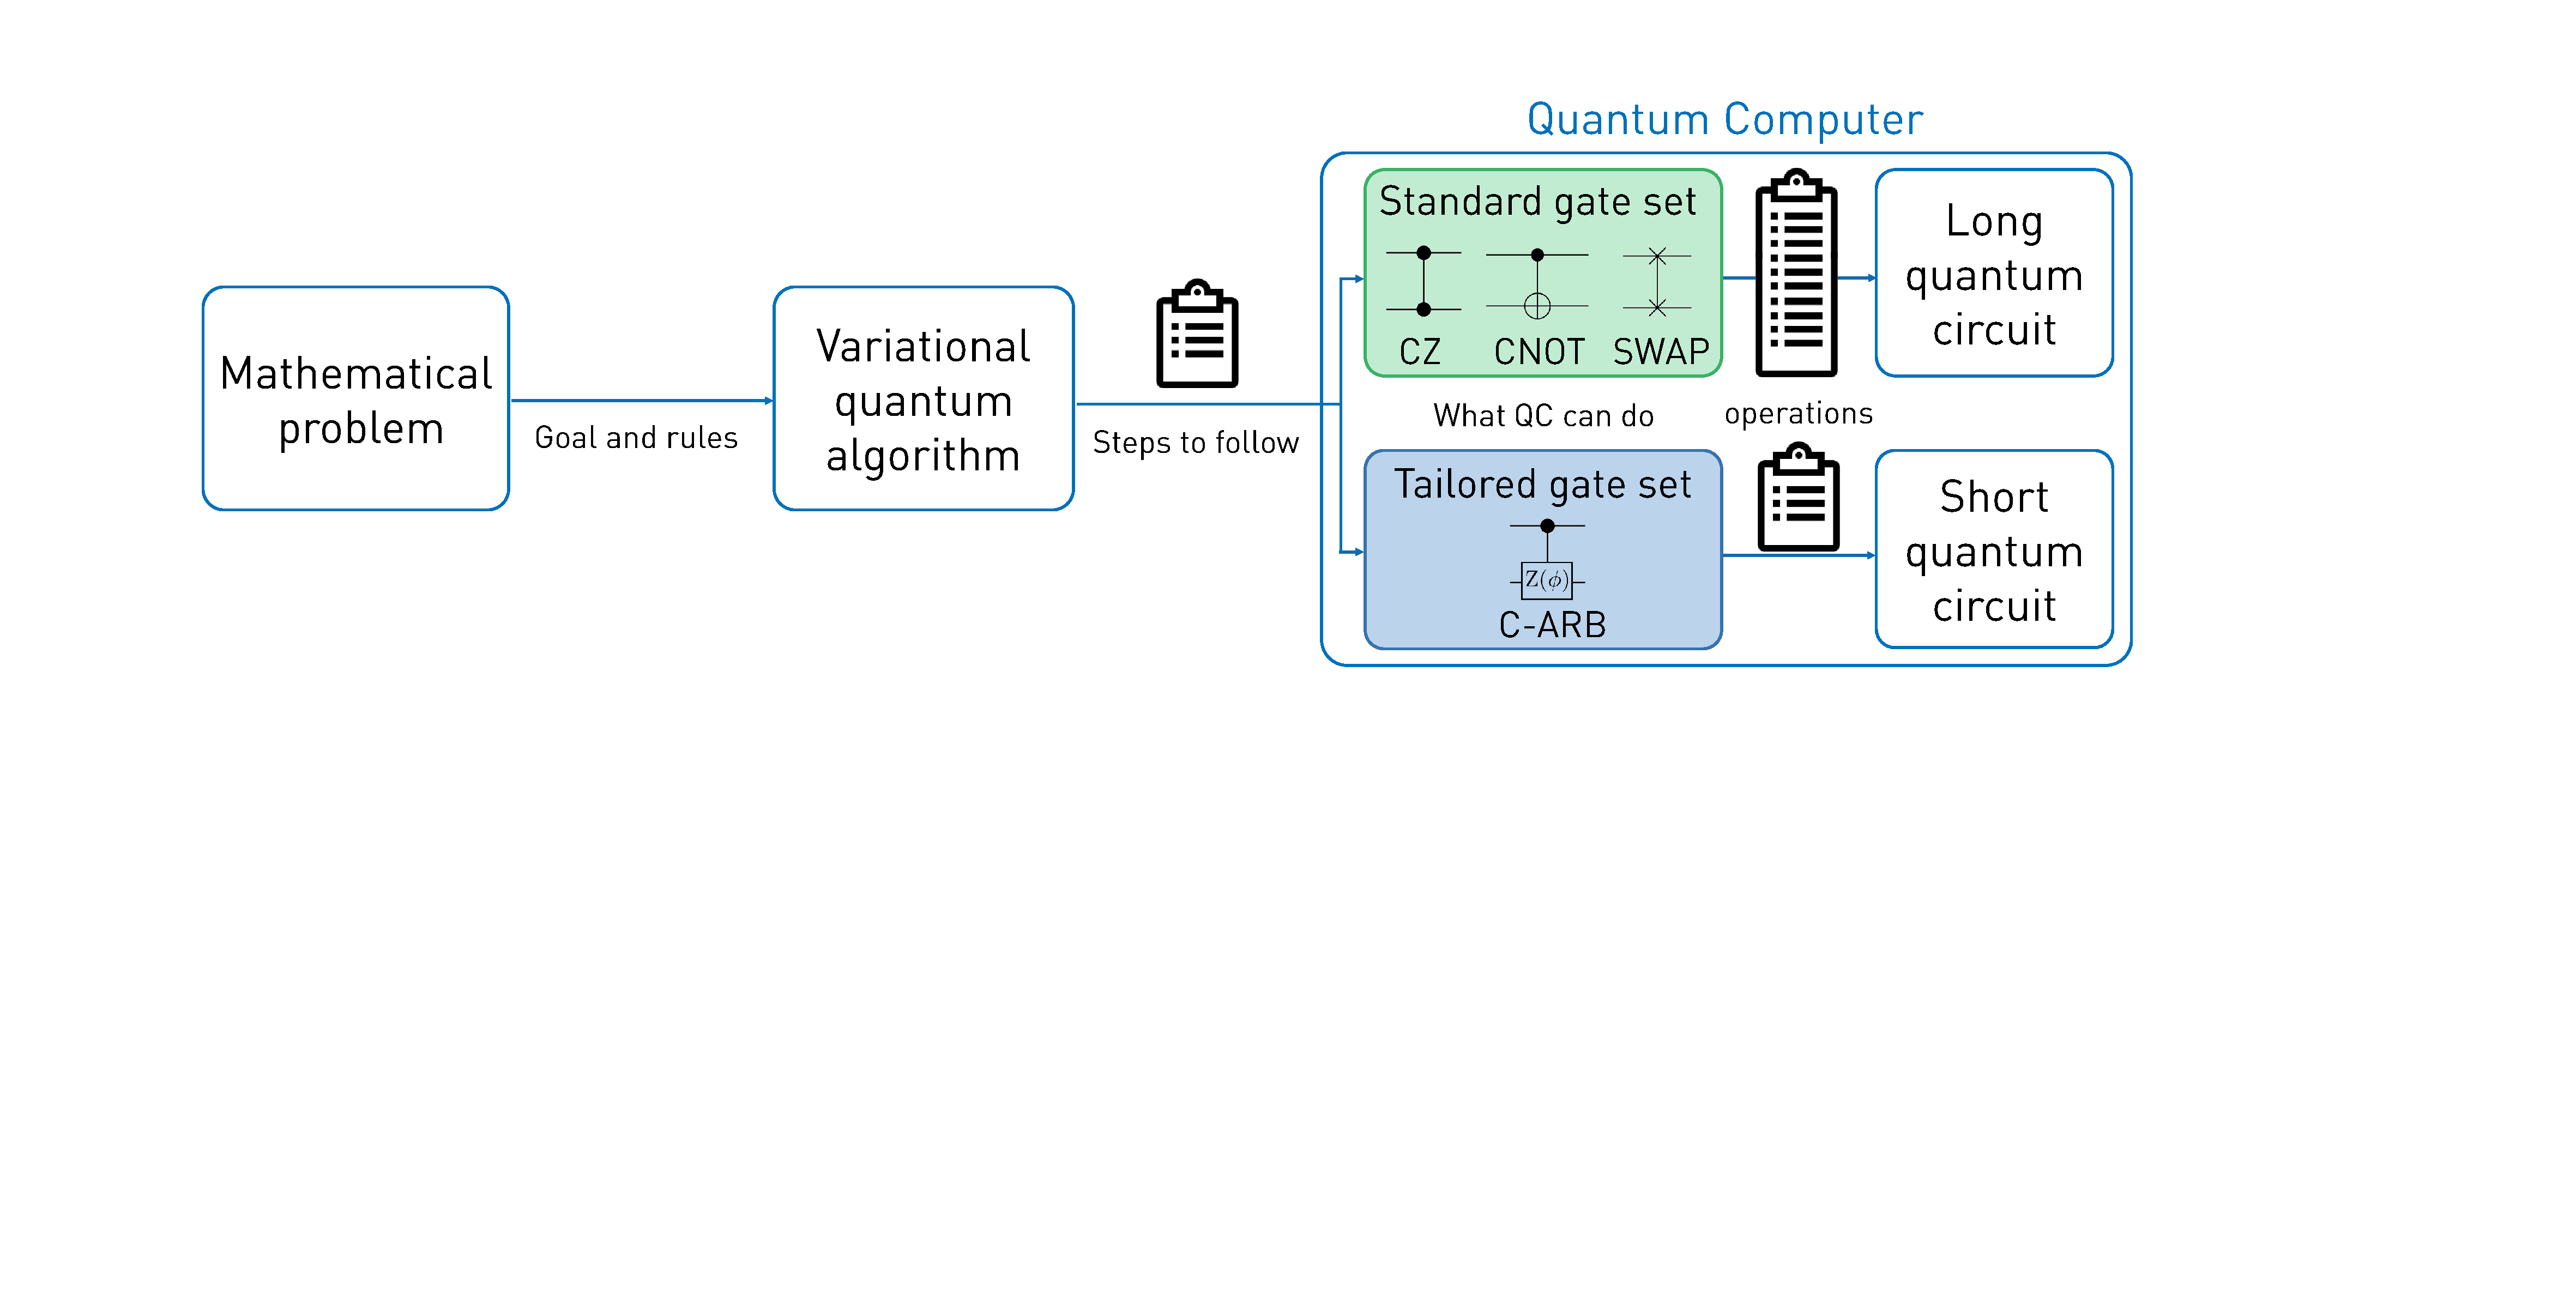
\includegraphics[width=\textwidth, trim={5cm 18cm 10cm 2cm},clip]{quantum_circuits_v3.pdf}
    \caption{Conceptual process flow to generate quantum circuits.}
    \label{fig:intro_quantum_circuits}
\end{figure}%\todo{harmonize color with vqa figure}

In this thesis, we present and characterize the \gls{carb}, an expressive two-qubit gate which avoids decomposition of instructions for various \glspl{vqa}. In the next section, we detail the basic working principle of \glspl{vqa} and explain why \glspl{carb} reduces the depth of their quantum circuits implementations.

\section{Variational quantum algorithms}
\glsreset{vqa}
\Glspl{vqa} encompass hybrid quantum-classical algorithms which leverage a quantum computer prepare a state in a large state space that would be exponentially hard to prepare classically, while the rest of the computation is executed by a classical computer~\cite{Moll2017QuantumDevices}. The two most prominent \glspl{vqa} are the \gls{vqe}~\cite{Peruzzo2014AProcessor}, which finds approximate solutions to quantum chemistry problems and the \gls{qaoa}~\cite{Farhi2014AAlgorithm}, which applies to generic combinatorial optimization problems. Their basic working principle is illustrated in Fig.~\ref{fig:intro_vqa}.

\begin{figure}[b]
    \centering
    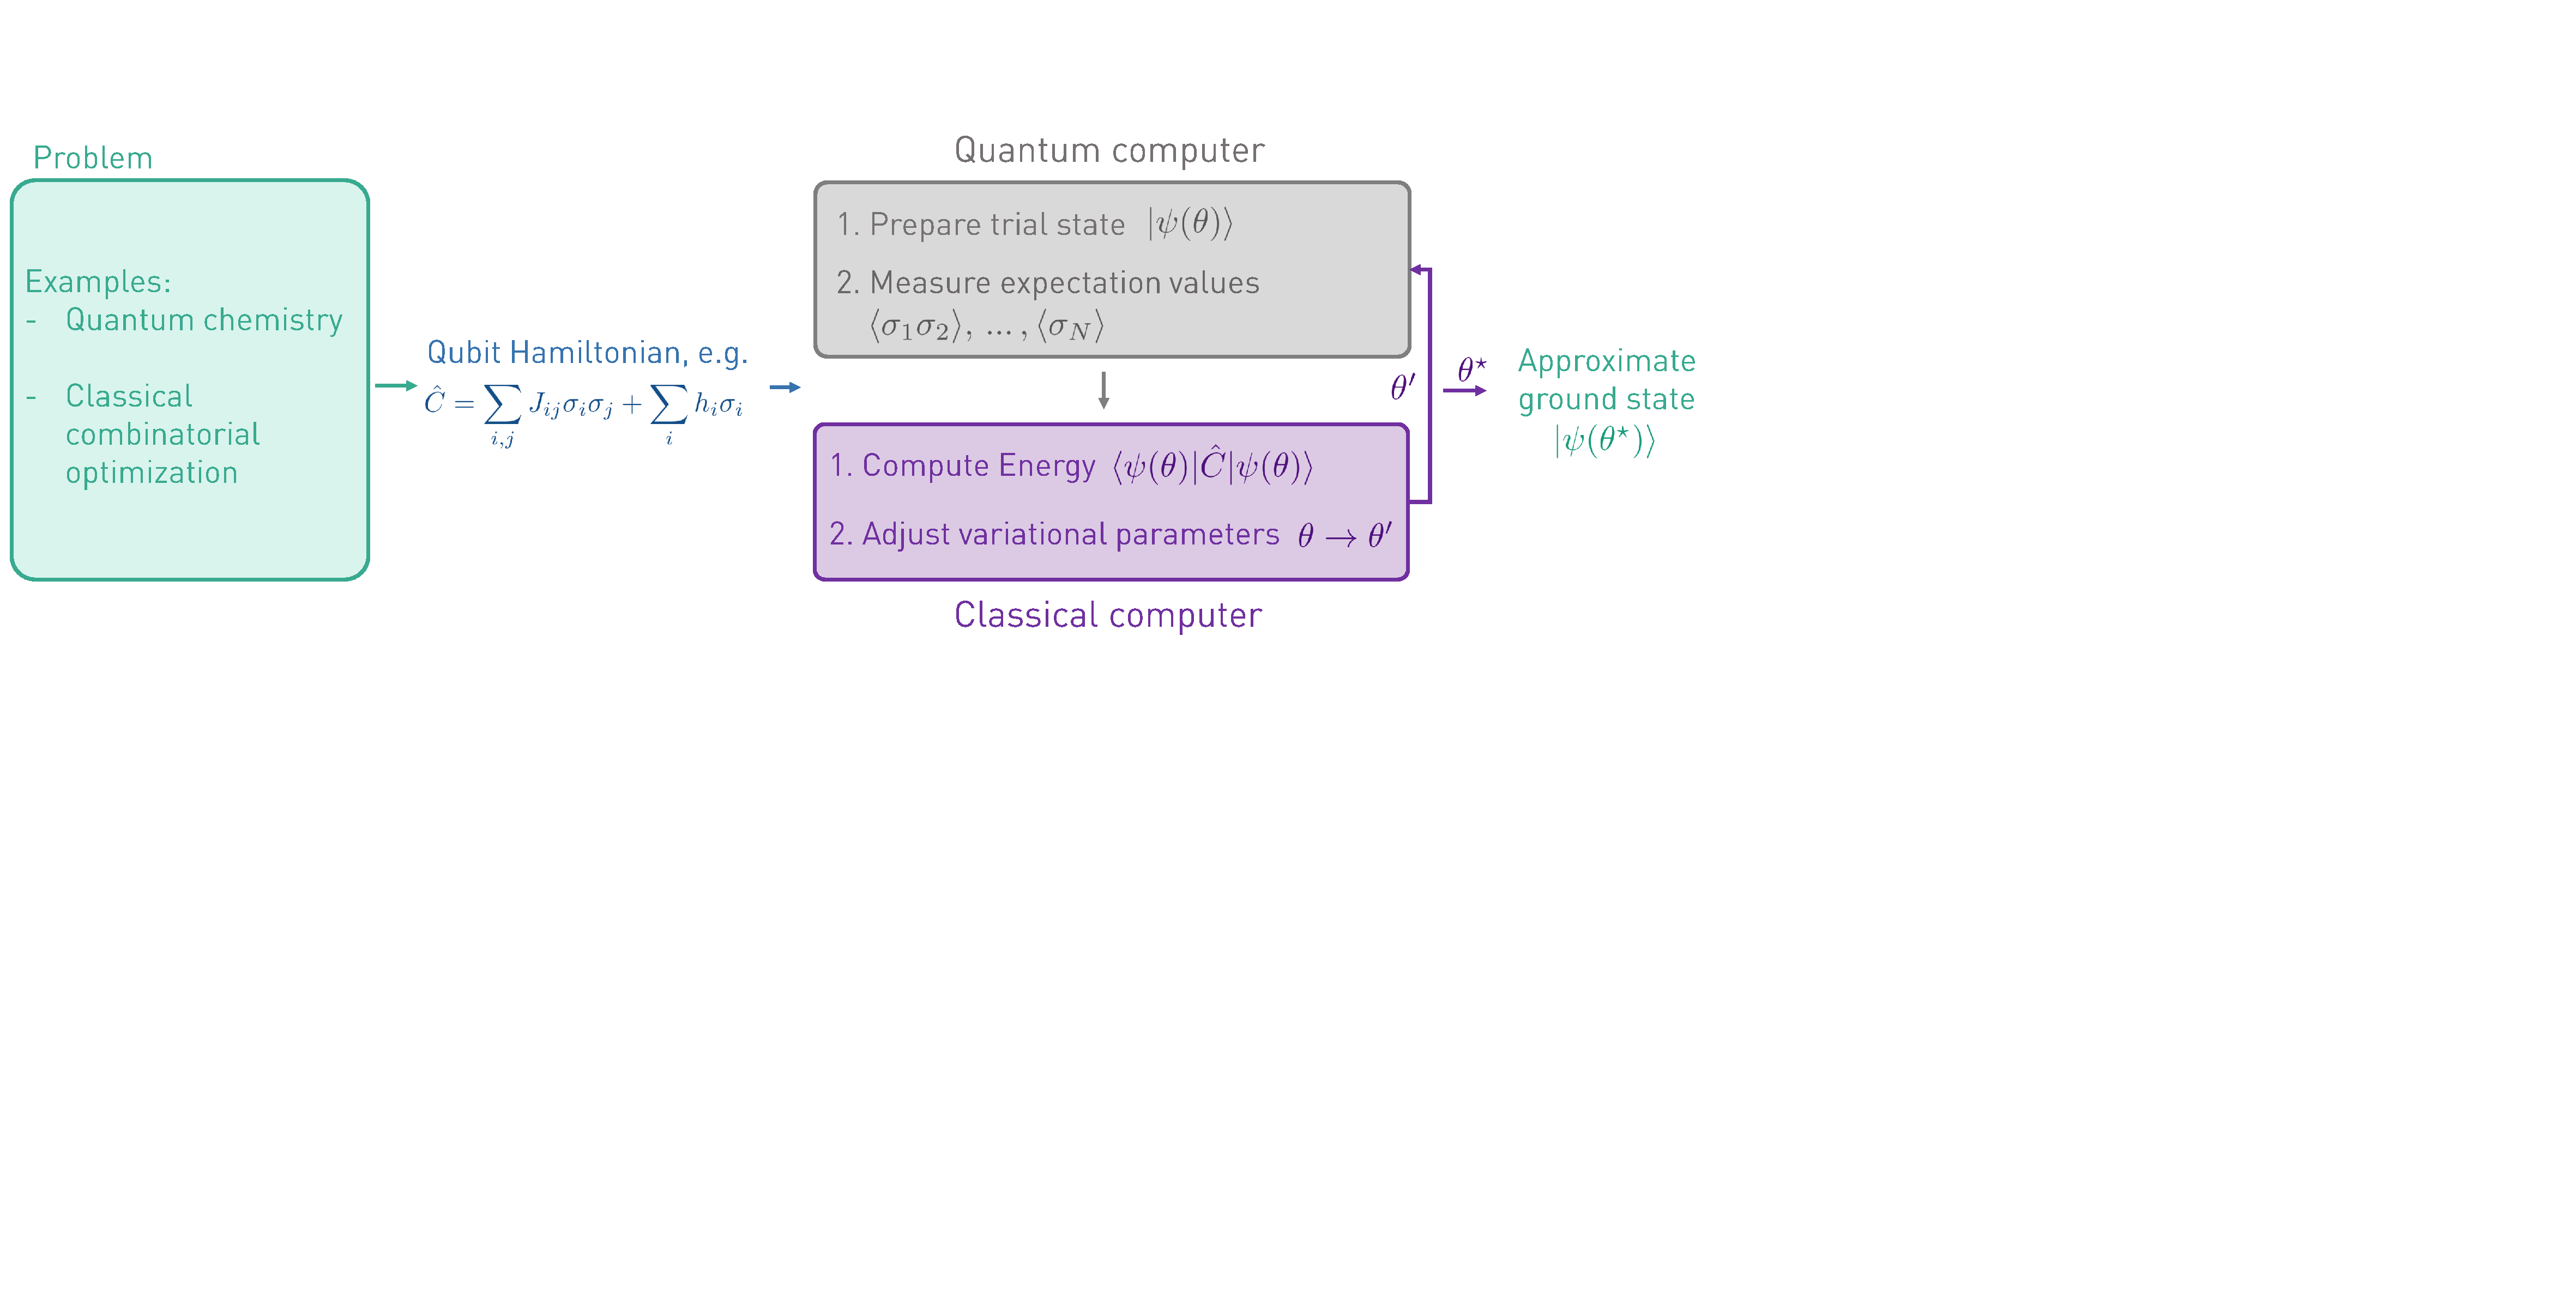
\includegraphics[width=\textwidth, trim={0cm 18cm 26cm 2cm},clip]{variational_quantum_algorithms_v2.pdf}
    \caption{Basic principle of a \gls{vqa}. A problem is mapped onto a qubit (cost) Hamiltonian $\hat C$,  where each term consists of tensor-products of individual Pauli operators~\cite[p.~65]{Nielsen2000QuantumInformation}. In this case, we picture an Ising-like Hamiltonian. The quantum computer prepares a parametrized trial state, $\ket{\psi(\theta)}$ and measures the expectation values of each term in $\hat C$. Based on the expectation value of the cost Hamiltonian, $\langle \psi(\theta) | \hat C |  \psi(\theta) \rangle$ a classical computer adjusts the circuit parameters, $\theta$, to minimize $\langle \hat C \rangle$.}
    \label{fig:intro_vqa}
\end{figure}

For both algorithms, the original problem is mapped in polynomial time to a (qubit) cost Hamiltonian, $\hat C$, such that its solution coincides with finding the ground-state energy of that Hamiltonian. Thereafter, the search for the ground-state is performed using both a quantum and a classical computer. 

The quantum computer generates a trial state $|\psi(\theta)\rangle$ based on variational parameters $\theta$ and the cost Hamiltonian. Repeated single shot measurements allow to estimate the expectation values for each term of the cost Hamiltonian. Based on the expectation value of the total energy, $\langle \psi(\theta) | \hat C |  \psi(\theta) \rangle$,  a classical optimizer suggests new variational parameters $\theta'$ to minimize the smooth function of the expectation value of the energy. At convergence, the final state $\ket{\psi(\theta^\star)}$ with corresponding final variational parameters $\theta^\star$ constitutes an approximate solution for the ground-state, from which an approximate solution to the original problem is deduced. 

The quality of the approximation strongly depends on the depth of the  quantum circuits. Indeed, \glspl{vqe} and \gls{qaoa} mimic a \textit{continuous} time evolution of the system with \textit{discrete} steps to find its ground-state~\cite{Lloyd1996UniversalSimulators} (see Section~\ref{sec:qaoa_relation_to_adiabiatic_computing} for a detailed discussion about \gls{qaoa}'s relationship to the time evolution of a quantum system). Each additional layer -- or step -- in the quantum circuit improves the quality of the approximation but also increases the number of operations and hence the depth of the circuit. 

In \gls{qaoa}, each layer $l$ directly includes the unitary evolution due to the cost Hamiltonian for a time defined by the variational parameter $\theta_l$: $U_{C_l}(\theta_l) = \sexp{-\i\hat C \theta_l}$. When $\hat C$ is an Ising-like Hamiltonian in the $z$-basis~\cite{Lucas2014IsingProblems},  two-qubit terms in $\hat C$ result in unitaries of the form $\sexp{-\i\,\phi}$ where $\phi = \theta_l\sigma_i^z\sigma_j^z$. Since the parameter $\theta_l$ can adopt continuous real values, the operation includes the addition of an (arbitrary) phase $\phi$ on the two-qubit state $\ket{11}_{ij}$, which cannot be implemented with a standard \gls{cz} which adds a $\pi$ conditional phase. Therefore, early implementations of \gls{qaoa} decomposed two-qubit terms into two two-qubit gates and additional single qubit gates (see Section~\ref{sec:qaoa} for more details). 

\section{Related work}
The idea of using expressive gate sets for \glspl{vqa} recently inspired research groups at IBM, Rigetti Computing and Google, see Table \ref{tab:qaoa_experiments}, entries 1-3. In 2019, Ganzhorn et al.\ implemented exchange-type gates tailored for quantum chemistry simulation~\cite{Ganzhorn2019Gate-EfficientComputer} with a fidelity of $\sim95\%$. In the same year, Abrams et al.\ implemented a more general XY-entangling gate~\cite{Abrams2019ImplementationPulse} with median fidelity of 97.4\%. This gate family directly applies to quantum chemistry simulations, and a combination of two gates of this family also reduces decomposition in quantum circuits for combinatorial optimization. Finally, Foxen et al.\ ~\cite{Foxen2020DemonstratingAlgorithms} implemented both an arbitrary iSWAP-type gate and an arbitrary conditional phase gate which they concatenate to achieve similarly general interactions as with the XY-entangling gate. They report a two-qubit Pauli error of $3.8\times 10^{-3}$.

All three research groups implemented gates for superconducting qubits. Ganzhorn et al.\ and Foxen et al.\ implemented tunable couplers-based gates~\cite{McKay2016UniversalBus, Chen2014QubitCoupling} while Abrams et al.\ realized parametric entangling gates~\cite{Reagor2018DemonstrationLattice} with one fixed and one tunable transmon.

At the time of writing, Abrams et al.\ is the only group that implemented the \gls{qaoa} using expressive gates~\cite{Abrams2019ImplementationPulse}. In combination with standard CZ-gates, their parametrized XY-gates enable an impressive two-qubit gate count reduction of $\sim$30\%, which they briefly illustrate for a one-layer \gls{qaoa} implementation of a four-qubit, all-to-all connected MaxCut problem graph.

However, several groups implemented the \gls{qaoa} with standard gates prior to Abrams et al.'s work, see Table \ref{tab:qaoa_experiments}, entries 4-6. In 2017, Otterbach et al.\ solved a clustering problem on 19 superconducting qubits~\cite{Otterbach2017UnsupervisedComputer}. The problem could be solved using a single layer of the \gls{qaoa} such that the decomposition -- which occurs in each layer -- did not strongly affect the performance of the algorithm. In 2019, Pagano et al.\ estimated the ground state energy of a transverse field Ising model with tunable long-range interactions with 20 trapped ions and a two-layer \gls{qaoa}~\cite{Pagano2019QuantumSimulator}. Similarly, the best theoretical approximate solution with two layers is only $\sim1.5\%$ away from the ground state with respect to the full energy scale. Bengtsson et al.\ were the first to implement a problem requiring a two-layer \gls{qaoa} on (two) superconducting qubits~\cite{Bengtsson2019QuantumProcessor}. 

\begin{table}
\small
\centering
\caption{Summary and comparison of publications on expressive gate sets (top three entries), \gls{qaoa} experiments (entries 4 to 6) and this work. Entries are ordered chronologically based on their publication date.}
\label{tab:qaoa_experiments}
\resizebox{\textwidth}{!}{%
\begin{threeparttable}
\begin{tabular}{ p{3.5cm} p{4cm} p{1.cm} p{2cm} p{1cm} p{4cm}}
\toprule
Authors & Main message & qubits & Problem  & layers\tnote{*}  & gate implementation \\ 
\midrule
Ganzhorn et al.~\cite{Ganzhorn2019Gate-EfficientComputer} & Exchange-type gates + VQE demo & 2 & H$_2$-molecular energy & - & parametric, tunable coupler based \\
Abrams et al.~\cite{Abrams2019ImplementationPulse} & XY-interaction gate family + QAOA demo & 4 & MaxCut & 1 (?) & parametric \\
Foxen et al.~\cite{Foxen2020DemonstratingAlgorithms} & Continuous SWAP and phase gates & 2 & - & - & tunable coupler based (gmon device) \\
\midrule
Otterbach et al.~\cite{Otterbach2017UnsupervisedComputer} & First QAOA implementation & 19 & MaxCut & 1 (1) & parametric CZ gates  \\
Pagano et al.~\cite{Pagano2019QuantumSimulator} & Analog implementation of Ising model with ions & up to 40 & Generic Ising & 2 (1) &  Analog long-range Ising \\ 
Bengtsson et al.~\cite{Bengtsson2019QuantumProcessor} & Solve a simple problem instance with high success probability using QAOA & 2 & Exact cover & 2 (2) &  parametric CZ gates with tunable coupler\\
\midrule
This work & Demonstrate the advantage of using \glspl{carb} for \gls{qaoa} & 3 & Exact cover & 9 (3) &  fixed coupling \glspl{cz} and \glspl{carb}\\
\bottomrule
\end{tabular}
\begin{tablenotes}
\item[*]Implemented layers and between brackets the number of layers required to solve the problem with a success probability larger than 95\%.
\end{tablenotes}
\end{threeparttable}}

\end{table}

In this thesis, we present the first in-depth experimental analysis of the advantage of expressive gates, i.e.\  \glspl{carb}, for the implementation of \glspl{vqa}. In Chapter \ref{ch:carb}, we describe the calibration and characterization procedure of a \gls{carb} for fixed-coupling, frequency-tunable transmons~\cite{DiCarlo2009DemonstrationProcessor} with an average process fidelity of $\sim 97.7\%$. In Chapter \ref{ch:qaoa}, we use \glspl{carb} to obtain a 50\% two-qubit gate count reduction on  a combinatorial problem exploiting the connectivity of our three-qubit device. We also implement for the first time a problem requiring three \gls{qaoa} layers to be solved with high success probability. In addition, we compare quantitatively on this problem the performance obtained with the direct implementation of the \gls{carb}, and its decomposed alternative. We show that, the \gls{qaoa} utilizing the direct implementation solves the problem with greater success probability. 
 